\documentclass[conference]{IEEEtran}

% Project paper prepared from the supplied IEEE conference template.
% Compile from this directory with: latexmk -pdf nlp_skill_pipeline_conference_paper_.tex
\usepackage{amsmath,amssymb,amsfonts}
\usepackage{graphicx}
\usepackage{url}
\usepackage{array}
\usepackage{booktabs}
\graphicspath{{./}}

\begin{document}

\title{NLP Techniques for Information Extraction and
Skill Taxonomy Construction from Unstructured
Job Advertisement Data}

\author{\IEEEauthorblockN{Tiago Luis Bispo Evangelista}
\IEEEauthorblockA{
\textit{Department of Computer Science \& Applied Physics} \\
\textit{Atlantic Technological University} \\
Galway, Ireland
}
}

\maketitle

\begin{abstract}
Job advertisements describe skills in variable, unstructured language, making it difficult to compare requirements across vacancies or connect employer terminology to a shared taxonomy. This paper presents an auditable pipeline that compares lexicon matching, noun-phrase generation with embedding retrieval, and supervised named-entity recognition (NER) followed by European Skills, Competences, Qualifications and Occupations (ESCO) ranking. Evaluation uses the SkillSpan test split and an availability-constrained Irish technology-posting corpus. The main Irish test set contains 85 annotated postings, 1,492 skill spans, and 1,404 URI-mapped units; 88 additional mentions are recorded as ESCO coverage gaps. The NER system achieves exact span F1 of 0.789 on SkillSpan, but 0.214 on the Irish test set. On the Irish set, the noun-phrase embedding baseline gives exact span F1 of 0.377, ESCO Acc@1 of 0.959, and at least one correct end-to-end output in 84 of 85 postings. The proposed NER pipeline reaches 0.785 Acc@1 but produces such an output in only 5 of 85 postings. A controlled encoder comparison favours MPNet over MiniLM. These results show that strong benchmark extraction and effective taxonomy ranking do not guarantee target-domain pipeline utility. We report separate extraction, linking, and coverage metrics, an aggregate trace-based error analysis, and an explicit account of corpus and denominator limitations.
\end{abstract}

\begin{IEEEkeywords}
skill extraction, job advertisements, named-entity recognition, ESCO, information extraction, domain transfer, evaluation
\end{IEEEkeywords}

\section{Introduction}
Job advertisements are a valuable source of evidence about employer demand, but they are written for people rather than for structured analysis. A single vacancy can mention programming languages, platforms, methods, qualifications, and interpersonal capabilities in prose that varies by employer, occupation, and source. Equivalent requirements may use different surface forms, while the same term may refer to a skill, a product, or general job context. Reliable analysis therefore requires identifying skill mentions in text and normalising them to concepts that can be compared across postings \cite{Khaouja2021,Rahhal2024,Senger2024}.

This paper studies that task as a pipeline with distinct stages. Extraction identifies a skill span and its boundaries. Taxonomy linking selects a canonical concept for that span. A system can succeed at one stage and fail at another: a correct phrase can receive a wrong concept, and a high-quality ranker cannot link a phrase that was never extracted. A single aggregate score obscures these differences. We therefore report span-level extraction, ESCO ranking, end-to-end posting coverage, and a trace-based error analysis separately.

The experiments compare three configurations. A lexicon baseline uses exact and fuzzy matching against English ESCO labels. An embedding baseline generates noun-phrase candidates and ranks ESCO concepts semantically. The proposed configuration applies a supervised NER model trained on SkillSpan, then generates candidates through a lexicon-first procedure with MPNet retrieval. ESCO provides the shared concept inventory and persistent identifiers needed for interoperable reporting \cite{ESCOPortal,ESCOClassification}.

The principal evaluation comprises 85 manually annotated Irish technology postings. These postings are part of a screened collection of 115 records across five entry-level role groups; 30 postings were reserved as an annotation pilot. The 85-posting test set is an availability-constrained sample and is not a probability sample of the Irish labour market. SkillSpan provides a separate external benchmark for extraction \cite{SkillSpan2022}. This design asks whether a model that performs well on that benchmark remains effective on the collected Irish material.

The findings differ by dataset and pipeline stage. The proposed NER system has the strongest extraction result on SkillSpan, with exact span F1 of 0.789. On the Irish test set, the embedding baseline has the strongest exact span F1 at 0.377 and the best ESCO scores over reviewed URI-mapped spans. It also achieves at least one correct complete output in 84 of 85 postings, compared with 5 of 85 for the automatic NER pipeline. This gap motivates a central conclusion: component performance must be interpreted alongside target-domain validation and posting-level coverage.

This paper makes four contributions. First, it describes an auditable implementation whose stages retain candidate lists, scores, methods, and failure reasons. Second, it compares three extraction and linking configurations across a benchmark and a geographically constrained external sample. Third, it exposes the difference between extraction quality, conditional taxonomy ranking, and end-to-end coverage. Fourth, it reports controlled ablations of embedding ranking, noun-phrase extraction, domain transfer, and encoder choice. The work is an evaluation of a defined research prototype; it does not claim national labour-market representativeness or production readiness.

\section{Related Work}
\subsection{Skill Extraction from Job Advertisements}
Research on skill identification in job advertisements spans dictionary matching, statistical methods, supervised sequence labelling, and more recent language-model approaches. Surveys describe a progression from manually curated vocabularies and text mining toward contextual models, while also noting that task definitions and datasets differ substantially \cite{Khaouja2021,Rahhal2024,Senger2024}. Lexicon methods remain interpretable and can work well when expressions closely match known labels, but synonymy, abbreviations, and compositional phrases limit exact matching \cite{Napierala2024,Ao2023}.

Supervised extraction depends on suitable span-level annotations. Green et al. introduced a benchmark resource for entity recognition in job descriptions, and SkillSpan provides English job-posting annotations for hard and soft skills \cite{Green2022,SkillSpan2022}. Contextual models can use surrounding words to disambiguate a phrase and predict boundaries, but their results are sensitive to the annotation scheme and the match between training and target domains. Work on German job advertisements demonstrates the value of fine-grained extraction and classification, while compositional annotation research argues that flat spans may not represent the relationships among a skill, a task, and an experience condition \cite{Gnehm2022,Kruger2025}.

Large language models and synthetic data have expanded the set of available extraction techniques. Studies have examined prompting, structured information extraction, and generated job postings for improving skill matching \cite{Nguyen2024,Howison2025,JobSkape2024}. These methods can reduce some annotation burdens but introduce new questions about consistency, verification, and reproducibility. The present study focuses on controlled lexicon, embedding, and supervised NER configurations, for which model inputs and outputs can be inspected directly.

\subsection{Taxonomy Linking and ESCO}
Taxonomies support consistent naming and exchange of labour-market information. ESCO represents skills, competences, qualifications, and occupations through concepts and identifiers, making it a practical European reference inventory \cite{ESCOPortal,ESCOClassification}. Its value does not imply complete lexical coverage: employer language may be new, local, overly broad, or more specific than available concepts. Recent work combines curated taxonomies with data-driven enrichment, multilingual representations, knowledge graphs, and expert validation to address emerging terminology and coverage \cite{Sleeman2018,ESCOXLMR2023,Kavas2025,DeSanto2026}.

Exact and fuzzy string matching offer a transparent starting point. Embedding retrieval can match semantically related phrases even when their surface forms differ. The resulting retrieval score is conditional on the span supplied to the ranker and on whether the correct concept exists among the candidates. ESCO linking should therefore report both the candidate-ranking metric and the extraction condition. Multilingual classification work further demonstrates that taxonomy alignment and occupational classification are related but distinct tasks \cite{Kavas2024,Gnehm2025}.

\subsection{Evaluation and Domain Transfer}
Comparisons across papers are difficult when corpora, labels, and metrics vary. Exact span matching penalises boundary differences; relaxed overlap measures whether a prediction reaches the correct phrase region. Token-level metrics provide another view, but none alone captures the correctness of the final canonical concept. Skill extraction studies increasingly call for evaluation that separates local extraction, classification, and downstream utility \cite{Senger2024,SkillSpan2022}.

Domain transfer is a particular concern for job advertisements. A benchmark and a target collection can differ in role mix, source, formatting, terminology, and annotation policy. The literature identifies domain adaptation and annotation quality as continuing challenges, and recent work on skill discovery highlights the role of expert validation when linking emerging expressions to taxonomies \cite{Napierala2024,DeSanto2026,Panzaru2025}. This study contributes a direct comparison of benchmark and Irish-sample extraction together with separate taxonomy and posting-level measurements.

\section{Research Questions}
The evaluation addresses four questions:
\begin{itemize}
  \item \textbf{RQ1:} Which extraction configuration produces the strongest span-level performance?
  \item \textbf{RQ2:} Which ESCO linking configuration produces the strongest ranked classification results?
  \item \textbf{RQ3:} Which error patterns most limit end-to-end performance?
  \item \textbf{RQ4:} How well does a model trained on SkillSpan generalise to the Irish job-posting sample?
\end{itemize}
These questions are comparative. They do not presume that the same model will be best under every dataset, metric, or use condition.

\section{Data and Annotation}
\subsection{SkillSpan Benchmark}
SkillSpan is used for model development and external extraction evaluation. The project copy contains 4,800 training rows, 3,174 development rows, and 3,569 test rows. The model interface converts the source annotations into BIO tags for two project classes. The source's \textsf{tags\_skill} is mapped to \textsf{SKILL\_TECH}, and \textsf{tags\_knowledge} is mapped to the secondary \textsf{SKILL\_TRANS} label. This is an operational mapping for the implemented classifier, not a claim that all source knowledge labels are interpersonal skills. Consequently, benchmark scores show performance under the project conversion and should not be interpreted as a direct estimate of performance under the Irish annotation policy.

\subsection{Irish Technology-Posting Sample}
The final screened Irish collection contains 115 postings: 24 cloud-support, 23 cybersecurity, 24 data-analyst, 21 quality-assurance, and 23 software-development records. Table~\ref{tab:corpus} shows how these records are divided between the pilot and main gold set. The 30-posting pilot is kept separate from the 85-posting main gold set. The pilot used six postings per role and achieved pre-adjudication token-level Cohen's $\kappa=0.7477$ after two annotators applied the v3 guide and an adjudicator resolved disagreements. The main test set contains 68,038 tokens and 1,492 annotated skill spans: 1,250 technical and 242 transferable-skill spans.

The final gold set yields 1,404 URI-mapped units for the reported ESCO ranking evaluation. A further 88 mentions are documented as ESCO coverage gaps and excluded from URI-ranking metrics. The distinction between a gold span and a URI-mapped unit is retained throughout. Neither the 85-posting set nor the 115-posting collection is treated as a representative sample of all Irish vacancies.

\begin{table}[!t]
\caption{Irish Sample Allocation}
\label{tab:corpus}
\centering
\small
\begin{tabular}{lrrr}
\toprule
Role group & Total & Pilot & Main gold \\
\midrule
Cloud support & 24 & 6 & 18 \\
Cybersecurity & 23 & 6 & 17 \\
Data analyst & 24 & 6 & 18 \\
Quality assurance & 21 & 6 & 15 \\
Software development & 23 & 6 & 17 \\
\midrule
Total & 115 & 30 & 85 \\
\bottomrule
\end{tabular}
\\[1mm]
\par\vspace{1mm}{\footnotesize Source: screened Irish posting inventory and final pilot/main-gold split.}
\end{table}

\subsection{Annotation Policy}
The Irish annotation guide uses a conservative boundary policy. Annotators label named tools, languages, platforms, standards, certifications, and technical methods as \textsf{SKILL\_TECH}. Explicit human capabilities, including communication and problem solving, are assigned \textsf{SKILL\_TRANS}. Job titles, recruitment boilerplate, generic duties, isolated verbs, and vague context words are labelled \textsf{O}. Annotators select the smallest complete concept, exclude wrappers such as ``experience with,'' and do not create overlapping or nested spans. When uncertain, the guide directs the annotator to use \textsf{O} and record the phrase for review. The approved guide and adjudication log are retained as project artefacts.

The two annotation classes are intended to distinguish technical requirements from explicit transferable capabilities. The boundary decision is deliberately stricter than a general relevance judgement: a phrase is not tagged merely because it sounds useful for a job. For example, a named platform is a technical skill, while a title such as ``Data Analyst'' is excluded even though it contains occupational terminology. Generic phrases such as ``work independently'' are not tagged unless they express an explicit capability under the guide. This policy makes the resulting spans more specific, but it also means that a model trained using another corpus's annotation conventions can be penalised for plausible but out-of-scope predictions.

\subsection{Annotation Agreement and Label Support}
The pilot's token-level Cohen's kappa was 0.7477 before adjudication. The two annotators and adjudicator resolved 244 disagreement groups covering 420 token disagreements. The adjudicator retained 135 annotator-1 decisions, retained 108 annotator-2 decisions, and added one explicit rule. Role-level kappa ranged from 0.6891 for software development to 0.8210 for data analysis. These figures document calibration on the pilot; they do not imply that the 85-posting evaluation was independently double annotated in full.

Table~\ref{tab:labels} reports BIO token counts for the main gold set. The counts include 1,250 technical spans and 242 transferable-skill spans. The 605 technical and 139 transferable continuation tokens indicate that a substantial part of the annotation consists of single-token spans, while compound requirements still require boundary prediction. The non-skill label accounts for the remaining 65,802 tokens, reflecting the sparse nature of span extraction in long-form advertisement text.

\begin{table}[!t]
\caption{BIO Label Counts in the Irish Main Gold Set}
\label{tab:labels}
\centering
\small
\begin{tabular}{lr}
\toprule
Label & Tokens \\
\midrule
\textsf{O} & 65,802 \\
\textsf{B-SKILL\_TECH} & 1,250 \\
\textsf{I-SKILL\_TECH} & 605 \\
\textsf{B-SKILL\_TRANS} & 242 \\
\textsf{I-SKILL\_TRANS} & 139 \\
\midrule
Total & 68,038 \\
\bottomrule
\end{tabular}
\\[1mm]
\par\vspace{1mm}{\footnotesize A B-label marks one annotated span. Source: \textsf{irish\_gold\_final.normalized.jsonl}.}
\end{table}

\section{Pipeline and Experimental Setup}
\subsection{Compared Configurations}
The system separates text preparation, extraction, candidate generation, ranking, and evaluation. The lexicon baseline normalises ESCO preferred and alternative labels, tries exact matching, and then applies fuzzy matching with a cutoff. It provides an interpretable reference with low computational complexity.

The embedding baseline forms contiguous noun-phrase candidates from the posting text and ranks the shared ESCO inventory by sentence-embedding similarity. Candidate windows are filtered using token and stopword rules. The similarity threshold was selected on development data. This configuration combines automatic candidate generation with semantic linking; its Irish extraction metrics and linking metrics are reported separately.

The proposed system applies a supervised transformer token classifier trained on the SkillSpan training split. Predicted BIO sequences are converted to skill spans. The linker first tries exact or fuzzy ESCO matching and supplements the list with MPNet similarity candidates when needed. The candidate record retains the URI, label, score, rank, and retrieval method. At inference, the system loads the saved NER checkpoint strictly rather than silently substituting a random model. The sentence vectors are normalised and searched using exact NumPy inner products, equivalent to cosine similarity for normalised vectors.

The configured NER base is JobBERT (\textsf{jjzha/jobbert-base-cased}). The recorded training configuration uses a learning rate of $3\times10^{-5}$, three epochs, maximum sequence length 128, weight decay 0.01, and seed 42. A requested batch size of 16 is implemented as per-device batches of at most four with gradient accumulation. The best checkpoint is selected on development F1. Inference uses the saved checkpoint and tokenizer, and the final evaluation uses a single retained model checkpoint. This paper therefore reports the measured checkpoint result rather than an average across multiple training seeds.

The lexicon and embedding rankers use the same local English ESCO inventory, which contains 15,163 skill records in the current project export. The lexicon index stores preferred and alternative labels under each concept URI. Exact normalised matches receive priority; when exact matching fails, fuzzy similarity is accepted only above a cutoff and subject to a shared-content-token rule. Embedding retrieval compares a span representation against the candidate matrix. The proposed system merges these sources, removes duplicate URIs, and returns up to five candidates. This design makes ranking decisions inspectable and allows the ablations to remove or substitute one component at a time.

Candidate generation differs between the two automatic extraction baselines. The embedding baseline forms contiguous token windows up to five tokens long and filters windows that begin or end with stopwords or contain too many function words. The supervised NER system produces boundaries from contextual token labels. Consequently, their candidate sets differ before ESCO ranking begins. This is why extraction metrics and reviewed-span linking metrics are separated: a ranker comparison over gold spans controls for candidate quality, while end-to-end coverage includes candidate generation and extraction.

Figure~\ref{fig:architecture} summarises the implemented alternatives and the shared ranking and audit stages.

Each processing stage produces an inspectable intermediate representation rather than a single opaque label. Text preparation preserves the source posting identifier and token offsets; extraction emits span text, label, and boundary; candidate generation and ESCO retrieval retain the candidate URI, preferred label, similarity or lexical score, rank, and method. The trace makes it possible to distinguish a missed span from a wrong URI and a no-candidate event from a low-ranked candidate. This separation is useful for error attribution, but it also means that records from different stages have different units of analysis. The paper therefore names the unit and denominator whenever a metric changes from tokens to spans, concepts, postings, or trace records.

The ESCO inventory is held constant for the main linking comparison. The local English export provides a fixed candidate universe for the experiments, so differences among the rankers are not caused by querying a changing online service. URI persistence also makes manual review auditable: a label can be revised without losing the identity of the concept. However, the inventory snapshot and the label index are not equivalent to a complete semantic model of ESCO. In particular, the experiment represents concepts through preferred and alternative labels and sentence embeddings, not a full graph of concept relations, scope notes, and occupational associations. Findings about ranking apply to this implemented representation.

\begin{figure*}[!t]
\centering
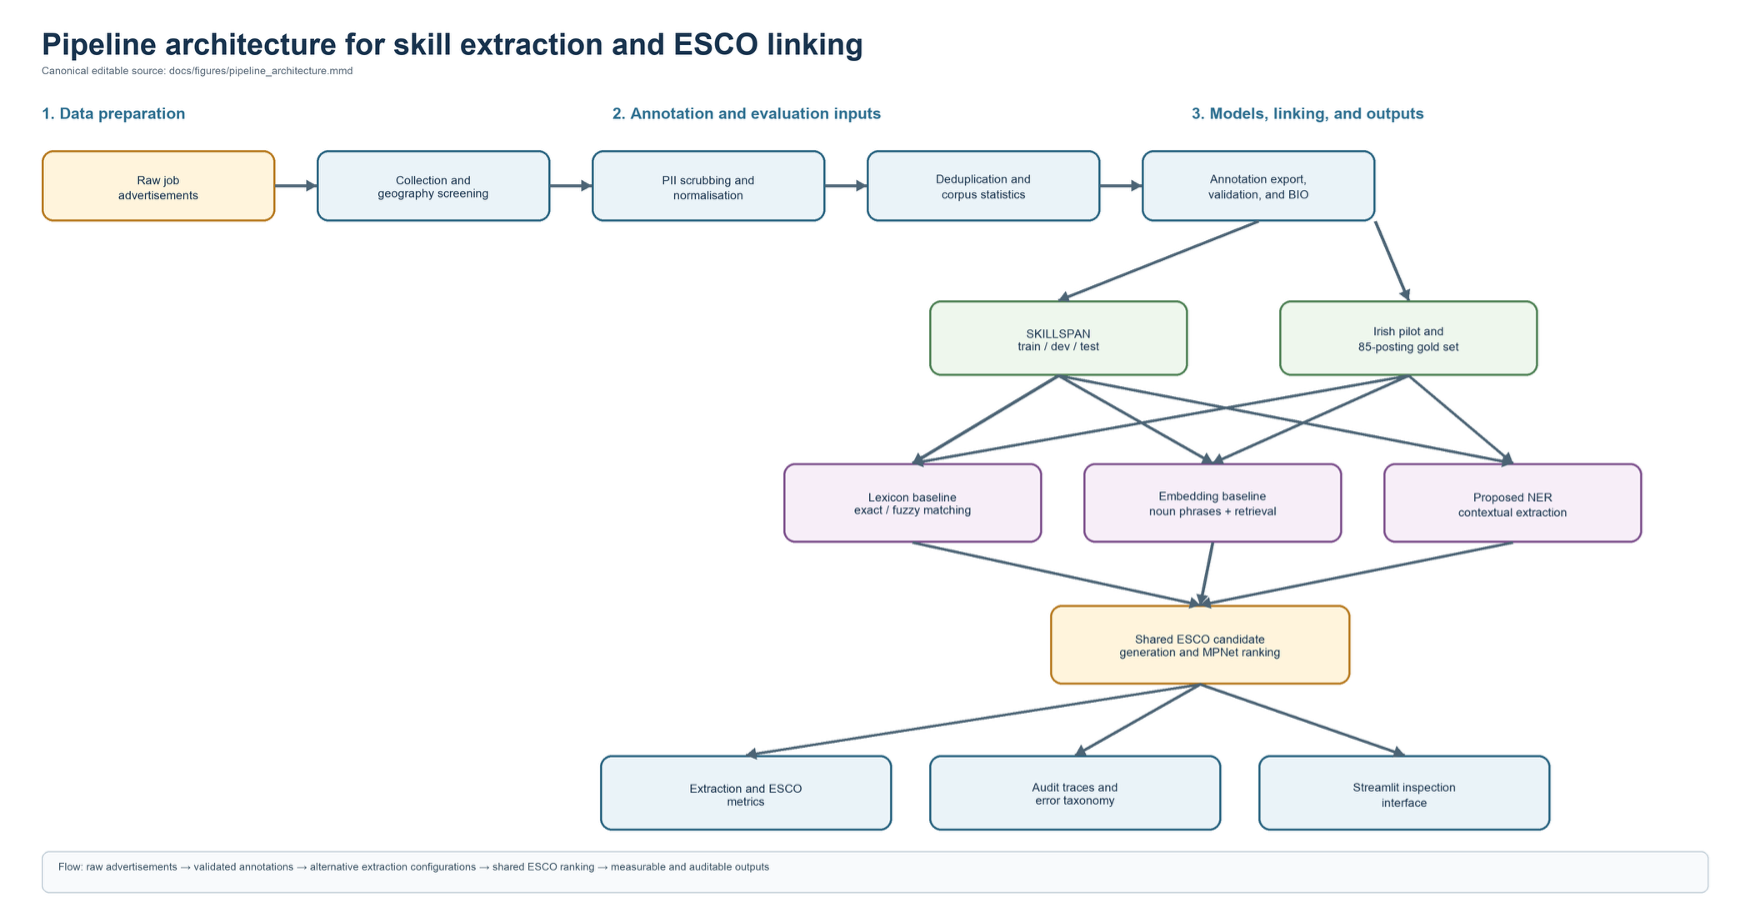
\includegraphics[width=0.98\textwidth]{pipeline_architecture.png}
\caption{Implemented pipeline from screened advertisements and annotations through alternative extraction systems, shared ESCO ranking, and audit outputs.}
\label{fig:architecture}
\end{figure*}

\subsection{Metrics and Denominators}
Extraction uses precision, recall, and F1 for exact span matching and relaxed overlap matching. Exact matching requires identical gold and predicted boundaries. ESCO linking uses Acc@1, Acc@3, mean reciprocal rank (MRR), and macro F1 over gold units with reviewed URIs. The reported Irish ESCO denominator is 1,404 units; 88 coverage-gap mentions are excluded. Posting coverage is the fraction of postings for which the configuration produces at least one correct end-to-end output. It does not measure the proportion of all skill mentions recovered in a posting.

For controlled linking comparison, all systems use the same reviewed gold units and the same ESCO inventory, while extraction metrics measure the span generator separately. This isolates ranking quality from extraction quality but means that an ESCO score alone is not a full automation score. SkillSpan and Irish results are kept as separate domains. We do not claim statistical significance because the work reports a single trained checkpoint and one availability-constrained test collection; confidence intervals and multi-seed variation remain future work.

For exact span evaluation, a predicted item is correct only when its start, end, and label match a gold span. Relaxed span evaluation counts labelled overlap and therefore gives a different view of boundary quality. For the ranked taxonomy metrics, let $r_i$ be the rank of the gold URI for reviewed unit $i$. Acc@$k$ is the proportion of units for which $r_i\leq k$, and MRR is the mean of $1/r_i$ with zero assigned when the URI is absent. End-to-end coverage counts a posting as covered when at least one candidate is both an exactly extracted gold span and linked to that span's reviewed URI. This strict conjunction makes coverage a useful system-level complement to local component metrics.

The denominators have distinct meanings. The 85-posting extraction evaluation includes all annotated tokens and spans. URI-linked ranking uses 1,404 reviewed units. The remaining 88 spans are reported as taxonomy coverage gaps, not as ranking misses. The integration gate is a separate 20-posting execution sample. The trace-based taxonomy counts 8,231 records in the Irish audit output and is a record-level error composition measure; its percentages are not a prevalence estimate over all postings or all gold spans.

Exact and relaxed scores answer different questions. Exact span F1 is the stricter measure for downstream indexing because a boundary error can change the concept phrase that is sent to the linker. Relaxed overlap is diagnostic: it reveals whether predictions reach the relevant region even when they include surrounding words or truncate a multi-token expression. A relaxed match should not be read as a fully correct extraction. The project also exports a field named \textsf{token\_f1}, but its implementation calls SeqEval's sequence-label precision, recall, and F1 functions. We therefore label these values as reported SeqEval scores, not token-wise accuracy, and do not substitute them for exact boundaries. The metrics are kept separate rather than combined into a new composite score.

The linking evaluation is conditional by design. Each of the 1,404 URI-mapped gold mentions is presented to each ranker, which makes the candidate-order comparison controlled with respect to the input phrase. The result estimates how often the correct reviewed URI is returned near the top when a gold phrase is supplied. It does not estimate the probability that an end-to-end system will first discover that phrase in unseen text. Posting-level coverage addresses a different, deliberately modest condition: whether any exact gold span in a posting is paired with its reviewed URI. It can therefore be high even when many mentions are missed, and low when a system extracts useful candidates but fails one stage of the exact-match conjunction.

No significance tests are presented. The Irish set is a finite, availability-constrained project sample, and only one retained NER checkpoint is reported. Treating individual spans as independent observations would overstate the effective sample size because multiple spans occur in the same posting and share source and role characteristics. Future statistical comparisons should use posting-level resampling or another clustered method, report uncertainty intervals, and ideally repeat model training across seeds. The current tables are descriptive measurements of the retained artifacts.

\subsection{Ablations and Integration Check}
Four analyses isolate pipeline choices. A1 removes embedding ranking while retaining the NER extractor and lexicon matching. A2 replaces NER predictions with noun-phrase candidates while retaining the ranker. A3 measures the difference between SkillSpan test and Irish gold extraction. A4 compares \textsf{all-mpnet-base-v2} with \textsf{all-MiniLM-L6-v2} over the same reviewed URI-mapped units. The integration gate processes a role-stratified 20-posting sample, records per-posting traces, and checks for populated URIs and extraction failures.

\section{Results}
\subsection{Extraction}
Table~\ref{tab:irish-extraction} shows the three configurations on the Irish main gold set. The noun-phrase embedding baseline has the highest exact span F1 at 0.377, followed by the lexicon baseline at 0.337 and the proposed NER system at 0.214. Its exact recall is 0.949. The NER system reaches relaxed F1 of 0.344 and relaxed recall of 0.968, suggesting that it often covers the local region of a skill while producing boundaries that differ from the conservative annotation. Its relaxed precision is 0.209, greater than the embedding baseline's 0.093, but the number of false-positive candidates remains consequential.

\begin{table*}[!t]
\caption{Extraction Metrics on the 85-Posting Irish Gold Set}
\label{tab:irish-extraction}
\centering
\small
\begin{tabular}{lrrrrrrl}
\toprule
Configuration & Exact P & Exact R & Exact F1 & Relaxed P & Relaxed R & Relaxed F1 & Evidence \\
\midrule
ESCO lexicon & 0.216 & 0.769 & 0.337 & 0.039 & 0.838 & 0.074 & 85 postings \\
Noun phrase + embedding & 0.235 & 0.949 & 0.377 & 0.093 & 1.000 & 0.169 & 85 postings \\
NER + MPNet ranking & 0.133 & 0.545 & 0.214 & 0.209 & 0.968 & 0.344 & 85 postings \\
\bottomrule
\end{tabular}
\\[1mm]
\par\vspace{1mm}{\footnotesize Source: corrected Irish results in \textsf{final\_results\_table\_irish.csv}.}
\end{table*}

On SkillSpan test, the order changes. Table~\ref{tab:skillspan} shows that the proposed NER system reaches exact span F1 of 0.789 and relaxed F1 of 0.906, exceeding the embedding baseline (0.639 and 0.370) and lexicon baseline (0.389 and 0.091). Its reported SeqEval F1 is 0.532; the source CSV calls this field \textsf{token\_f1}, although the implementation uses SeqEval's sequence-level scorer. The proposed system is strongest on the external benchmark under the project label conversion, but that result does not predict the same performance on the Irish sample.

\begin{table}[!t]
\caption{SkillSpan Test Extraction F1}
\label{tab:skillspan}
\centering
\small
\begin{tabular}{p{2.5cm}rrr}
\toprule
Configuration & SeqEval F1* & Exact F1 & Relaxed F1 \\
\midrule
ESCO lexicon & 0.014 & 0.389 & 0.091 \\
Noun phrase + embedding & 0.120 & 0.639 & 0.370 \\
NER + MPNet ranking & 0.532 & 0.789 & 0.906 \\
\bottomrule
\end{tabular}
\\[1mm]
\par\vspace{1mm}{\footnotesize Source: \textsf{final\_results\_table\_irish.csv}, SkillSpan test rows. *The exported \textsf{token\_f1} field is calculated with SeqEval's sequence-level scorer, not token-wise accuracy.}
\end{table}

Table~\ref{tab:class-f1} records the per-label SeqEval values exported by the project. They are included as an audit diagnostic, not as class-wise exact-span scores. The evaluation artifacts show a substantial discrepancy between this sequence-report path and the separate span scorer: on SkillSpan, SeqEval F1 is 0.532 while exact span F1 is 0.789; on Irish gold, the corresponding values are 0.0017 and 0.214. This cannot be explained by rounding. The per-label Irish values (0.0008 for \textsf{SKILL\_TECH} and 0.0029 for \textsf{SKILL\_TRANS}) should therefore not be used to claim a class-specific span-transfer rate. The discrepancy warrants an audit of the serialized labels, offsets, and scorer inputs; the current evidence does not identify which component causes it. The main extraction comparisons in this paper rely on the custom exact and relaxed span metrics, while the SeqEval fields remain transparently reported but are excluded from those conclusions.

\begin{table}[!t]
\caption{Proposed NER Per-Label SeqEval F1 (Diagnostic Output)}
\label{tab:class-f1}
\centering
\small
\begin{tabular}{lrr}
\toprule
Label & SkillSpan test & Irish main gold \\
\midrule
\textsf{SKILL\_TECH} & 0.4433 & 0.0008 \\
\textsf{SKILL\_TRANS} & 0.6137 & 0.0029 \\
\bottomrule
\end{tabular}
\\[1mm]
\par\vspace{1mm}{\footnotesize Source: per-label SeqEval report fields in the final extraction results; these are not class-wise exact-span F1 scores.}
\end{table}

The baseline ranking changes with the chosen evaluation condition. On the Irish corpus, noun-phrase generation obtains the strongest strict span F1, while the lexicon has lower exact recall but substantially fewer generated candidates. The NER system's relaxed recall is high, yet its strict precision is lowest. This is not a contradiction: relaxed matching can reward predictions that overlap a gold phrase, while exact evaluation rejects a boundary extension, a partial phrase, or an incorrect label. For a downstream taxonomy lookup, such boundary differences matter because the ranker receives a different string. The result argues for retaining both strict end-to-end measures and overlap diagnostics when comparing candidate generators.

\subsection{ESCO Linking}
Table~\ref{tab:esco} reports ranking on the 1,404 URI-mapped Irish evaluation units. The noun-phrase embedding baseline gives the highest Acc@1, Acc@3, and MRR: 0.959, 0.989, and 0.974. The proposed NER-plus-MPNet configuration reaches 0.785, 0.980, and 0.884. Its Acc@3 is close to the baseline, while its lower Acc@1 and MRR indicate that the correct concept is more often present among the candidates than selected at rank one. The lexicon baseline reaches 0.184 on all three metrics.

\begin{table}[!t]
\caption{ESCO Linking on Reviewed Irish Units}
\label{tab:esco}
\centering
\small
\begin{tabular}{lrrr}
\toprule
Configuration & Acc@1 & Acc@3 & MRR \\
\midrule
ESCO lexicon & 0.184 & 0.184 & 0.184 \\
Noun phrase + embedding & 0.959 & 0.989 & 0.974 \\
NER + MPNet ranking & 0.785 & 0.980 & 0.884 \\
\bottomrule
\end{tabular}
\\[1mm]
\par\vspace{1mm}{\footnotesize $N=1{,}404$ URI-mapped units; 88 coverage gaps excluded. Source: corrected Irish result table.}
\end{table}

The ESCO values are conditional on reviewed spans and URI availability. The high score for the noun-phrase baseline does not mean that its phrase candidates are all correct, nor that every skill in a posting is recovered. It describes ranking quality under the reviewed concept denominator. MPNet also outperforms MiniLM in the controlled encoder comparison: MiniLM-minus-MPNet deltas are $-0.412$ Acc@1, $-0.352$ Acc@3, $-0.375$ MRR, and $-0.512$ macro F1. The local index uses normalised embeddings and exact NumPy inner products, preserving cosine ranking without a separate approximate index.

\subsection{End-to-End Posting Coverage}
Table~\ref{tab:coverage} provides a stricter system-level view. At least one correct output is recorded for 49 of 85 postings with the lexicon system, 84 of 85 with noun-phrase embedding, and 5 of 85 with the proposed NER pipeline. These values correspond to coverage of 0.576, 0.988, and 0.059. Coverage is a low-threshold posting measure: one correct output is sufficient, so it should not be interpreted as complete extraction within a successful posting.

\begin{table}[!t]
\caption{End-to-End Posting Coverage}
\label{tab:coverage}
\centering
\small
\begin{tabular}{lrr}
\toprule
Configuration & Correct postings & Coverage \\
\midrule
ESCO lexicon & 49/85 & 0.576 \\
Noun phrase + embedding & 84/85 & 0.988 \\
NER + MPNet ranking & 5/85 & 0.059 \\
\bottomrule
\end{tabular}
\\[1mm]
\par\vspace{1mm}{\footnotesize Source: corrected end-to-end fields in the Irish results table.}
\end{table}

\subsection{Ablation Results}
The ablations in Table~\ref{tab:ablations} explain the different system outcomes. Removing embedding ranking (A1) leaves extraction unchanged but reduces the proposed system's Acc@1 by 0.601, Acc@3 by 0.796, and MRR by 0.700. Embeddings therefore provide most of the semantic ranking gain relative to exact or fuzzy matching alone.

Replacing NER with noun-phrase candidates (A2) increases exact span F1 by 0.163 and posting coverage by 0.882, while relaxed span F1 decreases by 0.175. The A2 run records 80/85 covered postings (0.941), whereas the final aggregate table records 84/85 (0.988) for the embedding baseline. This four-posting discrepancy is unreconciled; the values are retained with their source-specific denominators and should not be treated as interchangeable. The A2 result still isolates a large extraction effect, but its exact coverage must be checked against the final trace aggregation before camera-ready submission. Its controlled ESCO scores match the ranker reference because both are measured using the same reviewed gold units. Broad noun-phrase enumeration raises exact span F1 and posting-level coverage in the ablation while generating many candidates that require filtering or review.

A3 measures a large extraction gap between SkillSpan test and Irish gold: 0.575 in exact span F1 and 0.562 in relaxed F1. These differences are descriptive comparisons across domains and do not isolate a single cause. In A4, MiniLM is weaker than MPNet on all reported linking measures. The best encoder decision and the best complete pipeline decision are therefore distinct: MPNet is the stronger ranker, but the proposed NER extractor remains the principal bottleneck on the Irish evaluation.

\begin{table*}[!t]
\caption{Ablation Deltas on the Corrected Irish Evaluation}
\label{tab:ablations}
\centering
\small
\begin{tabular}{lrrrrrl}
\toprule
Ablation & Exact F1 $\Delta$ & Relaxed F1 $\Delta$ & Acc@1 $\Delta$ & Acc@3 $\Delta$ & MRR $\Delta$ & Comparison \\
\midrule
A1: remove embeddings & 0.000 & 0.000 & $-0.601$ & $-0.796$ & $-0.700$ & NER + lexicon vs full ranker \\
A2: noun phrase for NER & $+0.163$ & $-0.175$ & 0.000 & 0.000 & 0.000 & candidate generator substitution \\
A3: benchmark transfer & $+0.575$ & $+0.562$ & --- & --- & --- & SkillSpan test minus Irish gold \\
A4: MiniLM minus MPNet & --- & --- & $-0.412$ & $-0.352$ & $-0.375$ & same 1,404 reviewed units \\
\bottomrule
\end{tabular}
\\[1mm]
\par\vspace{1mm}{\footnotesize Sources: \textsf{ablation\_table\_irish.csv} and the A1--A4 JSON reports. Deltas follow each ablation's stated reference.}
\end{table*}

\section{Error Analysis and Integration}
The current Irish trace taxonomy contains 8,231 records, of which 8,226 are classified as errors. Table~\ref{tab:error-taxonomy} shows that false-positive extraction dominates (6,827; 82.99\%), followed by missed skill extraction (1,328; 16.14\%). Boundary errors account for 70 records (0.85\%); one soft-skill ambiguity is recorded (0.01\%). The audit records no E2 coverage-gap or E4 other-linking errors in this trace denominator. These trace labels are not the same as the separate manual ESCO review: that review contains 1,492 spans, including 88 without a suitable URI. We keep the two processes separate because the trace taxonomy counts prediction-level audit records, whereas the URI review classifies gold mentions.

The role breakdown also shows that false positives exceed missed spans in every group: the five role groups contribute 1,490/375 (cloud support), 1,623/297 (cybersecurity), 1,316/224 (data analysis), 1,142/202 (quality assurance), and 1,256/230 (software development), respectively. Raw counts should not be interpreted as role-specific error rates because postings and annotated span opportunities differ. The pattern is nevertheless consistent with the Irish NER results: relaxed recall is high (0.968), but exact precision is low (0.133), pointing to overinclusive or incorrectly bounded predictions as a dominant operational concern.

\begin{table}[!t]
\caption{Current Irish Trace-Error Taxonomy}
\label{tab:error-taxonomy}
\centering
\small
\begin{tabular}{llrr}
\toprule
Code & Error type & Count & Errors (\%) \\
\midrule
E1 & Boundary error & 70 & 0.85 \\
E2 & ESCO coverage gap & 0 & 0.00 \\
E3 & Soft-skill ambiguity & 1 & 0.01 \\
E4 & Other ESCO linking error & 0 & 0.00 \\
E5 & False-positive extraction & 6,827 & 82.99 \\
E6 & Missed skill extraction & 1,328 & 16.14 \\
\midrule
 & Total classified errors & 8,226 & 100.00 \\
\bottomrule
\end{tabular}
\\[1mm]
\par\vspace{1mm}{\footnotesize Percentages use the 8,226 classified errors; five additional trace records are marked correct. Source: current Irish trace audit.}
\end{table}

The error taxonomy is informative about where to intervene, but its categories need to be read at the right level. A false-positive trace means the system produced a span not supported by the corresponding gold annotation; it does not establish that the phrase is never useful to an employer. A missed-skill trace means a gold mention was not recovered by the audited extractor; it does not imply that the ESCO inventory lacks the concept. Boundary errors refer to partial or extended mentions. By separating these categories, the audit discourages a common but unhelpful response of treating every failure as a taxonomy lookup problem.

The false-positive concentration suggests beginning adaptation with hard negatives sampled from the same genres that trigger spurious predictions: introductory prose, generic responsibilities, experience wrappers, role titles, and common workplace language. These examples should be adjudicated rather than filtered solely by a broad stopword list, because relevant skill phrases may themselves contain common words. Missed mentions point toward collecting target-domain positive examples and inspecting the model's low-confidence regions. Boundary errors support adding compound spans and explicit wrapper examples to training and evaluation. The single recorded transferable-skill ambiguity is too sparse to justify a claim that this category is solved; targeted review should oversample such cases and report class-specific denominators.

The role-wise counts in Table~\ref{tab:role-errors} provide a descriptive check that false positives are not isolated to one role. Cybersecurity contributes the largest raw count of false-positive records, while cloud support has the largest missed count in this audit. Because the dataset allocates 15--18 main-gold postings per role and the counts are not normalised by eligible tokens or gold mentions, this ordering cannot be interpreted as comparative difficulty. It can, however, help prioritise a balanced sample for qualitative error review.

\begin{table}[!t]
\caption{False-Positive and Missed-Span Trace Counts by Role}
\label{tab:role-errors}
\centering
\small
\begin{tabular}{lrr}
\toprule
Role group & False positive & Missed skill \\
\midrule
Cloud support & 1,490 & 375 \\
Cybersecurity & 1,623 & 297 \\
Data analyst & 1,316 & 224 \\
Quality assurance & 1,142 & 202 \\
Software development & 1,256 & 230 \\
\bottomrule
\end{tabular}
\\[1mm]
\par\vspace{1mm}{\footnotesize Counts are audit records, not role-normalised rates. Source: current Irish trace audit.}
\end{table}

The Irish top-10 ESCO diagnostic in Fig.~\ref{fig:confusion} shows recurring semantically related but incorrect top-ranked concepts. Examples include predicting ``Kali Linux'' for ``operating systems'' and ``engage with stakeholders'' for ``communicate with stakeholders.'' These errors motivate contextual hard negatives and better concept descriptions. A confusion-pair frequency should not be read as the frequency of all extraction errors; it describes only the reviewed top-1 linking cases represented in the diagnostic.

\begin{figure*}[!t]
\centering
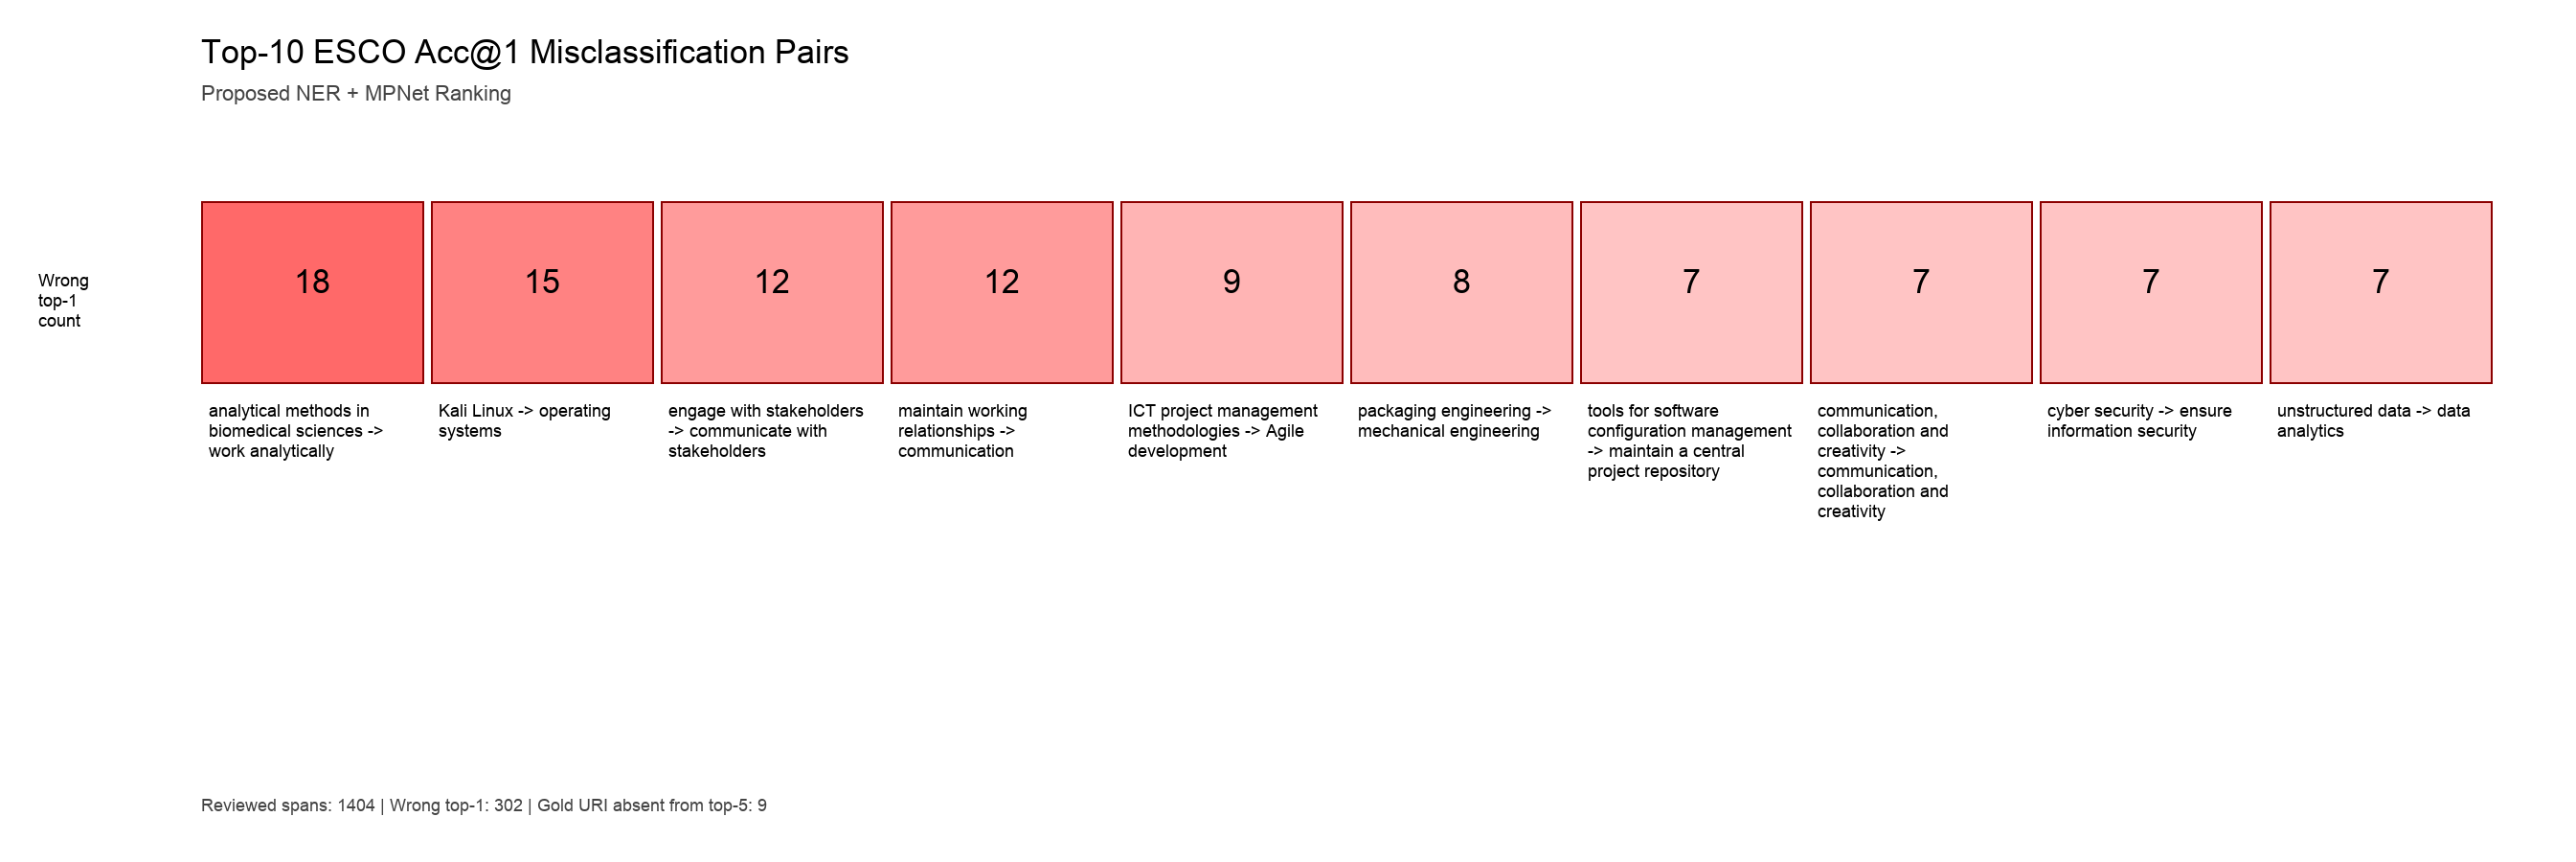
\includegraphics[width=0.98\textwidth]{figure2_confusion_irish.png}
\caption{Top-10 ESCO Acc@1 misclassification pairs among reviewed URI-mapped spans for the proposed NER and MPNet configuration. Only cases where the gold URI occurs in the retrieved top five are included; 1,404 reviewed units form the ranking denominator. Pair counts describe ranking confusions, not extraction errors or all taxonomy coverage gaps.}
\label{fig:confusion}
\end{figure*}

The integration gate ran the complete software path on 20 postings, wrote 20 trace files and 102 URI-populated prediction records, and flagged six postings with no detected spans. Execution and trace generation succeeded, but the warnings mean the gate was not a clean quality pass. Failures occurred in four of the five role groups, with three of the six in quality assurance. This check confirms that the modules can be joined and inspected while identifying an unresolved operational failure mode.

The integration result distinguishes software operability from model quality. A successful run demonstrates that the input can traverse preprocessing, extraction, ranking, and trace writing without a fatal exception; it does not show that every output is correct. Conversely, a no-span warning is not necessarily a crash: it is a valid but potentially harmful empty prediction that should be surfaced to a reviewer. The six warnings should therefore remain visible in demonstrations and future regression tests. An operational acceptance gate for this prototype should include both technical assertions (expected output schema, valid URI format, deterministic trace creation) and quality assertions (minimum recall on a labelled sample, maximum no-span rate, and reviewable confidence thresholds).

\section{Discussion}
\subsection{Answers to the Research Questions}
\textbf{RQ1: extraction.} The answer depends on the evaluation domain. The NER model is strongest on SkillSpan, but the noun-phrase embedding baseline has the strongest exact extraction F1 on the Irish gold set. NER's higher relaxed F1 than the Irish embedding baseline indicates overlap with gold skill regions, but exact boundaries and precision remain weak. The evidence supports supervised extraction when training and test conditions are aligned, and additional Irish calibration before automatic use in the target setting.

\textbf{RQ2: ESCO linking.} Semantic retrieval materially outperforms lexicon-only ordering. The noun-phrase embedding baseline achieves the strongest conditional Irish linking scores, while the proposed NER-plus-MPNet configuration is also strong at Acc@3. MPNet clearly outperforms MiniLM under the controlled encoder comparison. However, conditional linking metrics do not measure whether the extractor supplied appropriate spans.

\textbf{RQ3: errors.} The current Irish trace taxonomy is dominated by false-positive extraction (82.99\%) and missed skills (16.14\%), with boundary errors at 0.85\%. The separate manual review identifies 88 gold mentions without a suitable URI, but they are not counted in the trace-error denominator. The integration sample independently shows six no-span failures. Taken together, these measures suggest that improving extraction and confidence calibration is a higher immediate priority than expanding the ESCO inventory, while the 88 reviewed gaps remain a distinct taxonomy-maintenance concern.

\textbf{RQ4: generalisation.} The SkillSpan-trained model transfers poorly to the Irish sample under exact and relaxed span F1. The comparison cannot assign the decline to one factor because data source, role mix, formatting, and annotation policy change together. Still, the performance gap is large enough to show that external benchmark success cannot establish target-domain reliability.

\subsection{Practical Implications}
The experiments suggest a staged workflow for current use. Reviewed spans with MPNet retrieval provide the strongest reference for linking, while the NER-plus-MPNet design offers an auditable route to automatic extraction but should keep human review available. Candidate scores, alternate URIs, source context, and failure reasons should remain visible. The results do not support presenting the automatic NER system as production-ready for this Irish sample.

The distinction between retrieval and extraction also has implications for reporting. A score such as Acc@1 should identify its evaluation condition and denominator. A high conditional ranker score can coexist with low posting coverage if the upstream extractor fails. Likewise, a high posting coverage can coexist with poor span precision if only one correct output is required per posting. Reporting the three levels together provides a more faithful account of system behaviour.

For a researcher or analyst using the current implementation, the strongest immediate workflow is not to select one configuration as universally best. The noun-phrase embedding baseline offers broad recall and high measured posting coverage in this sample, but its candidate volume and exact precision imply substantial review burden. The lexicon is more transparent and can serve as a conservative anchor, but its semantic ceiling is visible in the linking scores. The NER pipeline gives a structured, learnable extraction stage and leads on SkillSpan, yet its Irish-target results and integration warnings make unattended use unjustified. A practical prototype can therefore expose multiple candidates and provenance, while requiring human confirmation for spans and URI decisions.

This human-review design is also a way to convert system uncertainty into useful project evidence. Reviewers can prioritise low-margin candidate lists, unseen phrases, transferable-skill expressions, and outputs near the span-boundary threshold. Corrections should be recorded as adjudicated examples with the same annotation policy used for test evaluation. If those cases later become training data, they must be separated from a future held-out test set to avoid optimistic reuse. A versioned review log can additionally distinguish genuine taxonomy gaps from extraction failures and ranking mistakes.

The results have a further implication for labour-market analysis: normalized skill counts are downstream estimates, not direct observations. Over-extraction can inflate demand for generic expressions, while under-extraction can hide niche or emerging capabilities. A wrong URI can merge distinct employer requirements or fragment one skill across several concepts. Any aggregate report should retain source, time, role, extraction version, URI, confidence, and review status. The current experiments do not estimate labour-market prevalence; they evaluate system behaviour on a limited sample. Keeping this distinction explicit protects downstream users from treating an experimental prototype as a census instrument.

Finally, the local ESCO inventory provides a reproducible reference point, but taxonomy versions should be recorded alongside results. New concept labels, alternate labels, and changes in URI status can alter retrieval even when the model weights remain fixed. A future benchmark release should package the exact inventory snapshot or its checksum, the annotation guide version, model checkpoint identifier, and evaluation scripts. Such provenance makes later changes traceable and helps explain why an apparently identical pipeline may yield different mappings when its reference inventory changes.

\subsection{Limitations}
The Irish sample is small, source-constrained, and limited to five entry-level technology roles. Results cannot be generalised to all Irish employers, occupations, seniority levels, or future vacancy language. The annotation scheme is flat and conservative; it does not represent relations among skills, tasks, tools, proficiency, or negation. The benchmark mapping from SkillSpan knowledge tags to the project secondary class adds a comparability caveat. Trace taxonomy percentages describe the current audit records, not the prevalence of errors in a population of advertisements. The four-posting mismatch between A2 coverage and the final embedding aggregate also requires reconciliation before these figures are used as a single canonical result.

The study reports one saved model checkpoint and does not provide a complete hyperparameter-search record or multi-seed uncertainty. The 1,404 URI-mapped linking denominator excludes 88 coverage gaps. The embedding baseline's component scores are conditional on reviewed gold spans, while its automatic noun-phrase generation can generate a large candidate set. Finally, the integration gate has six no-span cases. These limits narrow the deployment claims but do not erase the controlled evidence about model ranking and domain transfer.

There are also construct and measurement limitations. The two project labels compress a varied concept of skill into technical and transferable categories, while the flat BIO format cannot represent nested requirements, skill-task relations, negation, proficiency, or whether a requirement is mandatory or preferred. The ESCO URI review is a valuable adjudication layer, but mapping a phrase to one URI can be ambiguous when a posting phrase is broad or context-dependent. The metric treats the selected URI as a single gold answer even where several neighbouring concepts may be defensible. A future release could retain one primary URI and a documented set of acceptable alternatives, then report both strict and adjudicated-set retrieval scores.

Corpus construction introduces selection effects. The sample contains a screened set of records across five role families and includes postings from a limited set of sources; the pilot and main gold split are separated by posting, but the 85 postings are still not a random sample. Repeated templates, employers, or source-specific formatting may affect the apparent difficulty, and the current tables do not estimate those effects. The evaluation also excludes missing or unsuitable taxonomy mappings from ranking metrics, so Acc@k is conditional on the subset for which a URI was assigned. Reporting the 88 excluded mentions prevents denominator inflation but cannot remove this selection condition.

Reproducibility is bounded by local model and inventory artifacts. The configuration records the base model, seed, schedule, and principal sequence length, but one retained checkpoint does not quantify training variance. Exact retrieval avoids approximate-index randomness, yet library versions, tokenizer behavior, normalization, and the ESCO snapshot can still matter. The current study should therefore be read as a reproducible direction with recorded artifacts, not as a fully locked benchmark package. Before external release, hashes for model files and the ESCO export, a clean-install reproduction command, and a test of the stated result table should be checked together.

\section{Conclusion and Future Work}
This paper evaluated an auditable pipeline for extracting skill mentions from job advertisements and linking them to ESCO. The proposed NER model performs strongly on SkillSpan but loses substantial performance on the Irish sample. The noun-phrase embedding baseline achieves the strongest Irish exact span F1, conditional ESCO linking, and posting coverage. MPNet outperforms MiniLM in the controlled ranker comparison, and embedding ranking contributes a substantial improvement over lexicon-only linking.

The central result is that benchmark extraction, taxonomy ranking, and end-to-end utility measure different properties. The current evidence supports the pipeline as a research prototype and supports MPNet as the preferred encoder among those compared, while showing that Irish-domain extraction remains the limiting step. Future work should annotate a separate Irish development set, calibrate NER confidence, add difficult negative examples from generic recruitment language, and evaluate a retrained model on a held-out target-domain test set. It should also rebuild the trace taxonomy for the current Irish gold set, include adjudicated skill classes where supported, and report multi-seed variation and confidence intervals. Broader role and source coverage will be needed before making claims about the Irish labour market as a whole.

\appendices
\section{Project Repository}

Repository URL: \url{https://github.com/tiagoluis12/nlp-skill-pipeline}.

The repository provides source code, the conference paper, and aggregate evaluation artifacts. Original Irish job postings, annotations, and record-level predictions and traces are not included because redistribution permission for the source postings has not been established; the Irish experiments therefore cannot be rerun from a fresh clone. This publication uses the ESCO classification of the European Commission.

\begin{thebibliography}{00}
\bibitem{Khaouja2021} I. Khaouja, I. Kassou, and M. Ghogho, ``A survey on skill identification from online job ads,'' \emph{IEEE Access}, vol. 9, pp. 118134--118153, 2021, doi: 10.1109/ACCESS.2021.3106120.
\bibitem{Rahhal2024} I. Rahhal, I. Kassou, and M. Ghogho, ``Data science for job market analysis: A survey on applications and techniques,'' \emph{Expert Systems with Applications}, vol. 251, Art. no. 124101, 2024, doi: 10.1016/j.eswa.2024.124101.
\bibitem{Senger2024} E. Senger, M. Zhang, R. van der Goot, and B. Plank, ``Deep learning-based computational job market analysis: A survey on skill extraction and classification from job postings,'' in \emph{Proc. NLP4HR}, 2024, pp. 1--15, doi: 10.18653/v1/2024.nlp4hr-1.1.
\bibitem{Napierala2024} J. Napiera\l{}a, ``Enhancing taxonomy-based extraction: Leveraging information from online community platforms for digital skills demand identification in job ads,'' \emph{Statistical Journal of the IAOS}, vol. 40, no. 3, pp. 591--602, 2024, doi: 10.3233/SJI-230110.
\bibitem{Ao2023} Z. Ao, G. Horv\'ath, C. Sheng, Y. Song, and Y. Sun, ``Skill requirements in job advertisements: A comparison of skill-categorization methods based on wage regressions,'' \emph{Information Processing \& Management}, vol. 60, no. 2, Art. no. 103185, 2023, doi: 10.1016/j.ipm.2022.103185.
\bibitem{Green2022} T. A. F. Green, D. Maynard, and C. Lin, ``Development of a benchmark corpus to support entity recognition in job descriptions,'' in \emph{Proc. LREC}, 2022, pp. 1201--1208.
\bibitem{SkillSpan2022} M. Zhang, K. Jensen, S. Sonniks, and B. Plank, ``SkillSpan: Hard and soft skill extraction from English job postings,'' in \emph{Proc. NAACL-HLT}, 2022, pp. 4962--4984, doi: 10.18653/v1/2022.naacl-main.366.
\bibitem{Gnehm2022} A.-S. Gnehm, E. B\"uhlmann, H. Buchs, and S. Clematide, ``Fine-grained extraction and classification of skill requirements in German-speaking job ads,'' in \emph{Proc. NLP+CSS}, 2022, pp. 14--24, doi: 10.18653/v1/2022.nlpcss-1.2.
\bibitem{Nguyen2024} K. Nguyen, M. Zhang, S. Montariol, and A. Bosselut, ``Rethinking skill extraction in the job market domain using large language models,'' in \emph{Proc. NLP4HR}, 2024, pp. 27--42, doi: 10.18653/v1/2024.nlp4hr-1.3.
\bibitem{Kruger2025} K. Kr\"uger, J. Binnewitt, K. Ehmann, S. Winnige, and A. Akbik, ``Improving online job advertisement analysis via compositional entity extraction,'' in \emph{Proc. EMNLP}, 2025, pp. 27047--27065, doi: 10.18653/v1/2025.emnlp-main.1375.
\bibitem{Howison2025} M. Howison \emph{et al.}, ``Extracting structured labor market information from job postings with generative AI,'' \emph{Digital Government: Research and Practice}, vol. 6, no. 1, Art. no. 9, 2025, doi: 10.1145/3674847.
\bibitem{JobSkape2024} A. Magron, A. Dai, M. Zhang, S. Montariol, and A. Bosselut, ``JobSkape: A framework for generating synthetic job postings to enhance skill matching,'' in \emph{Proc. NLP4HR}, 2024, pp. 43--58, doi: 10.18653/v1/2024.nlp4hr-1.4.
\bibitem{ESCOPortal} European Commission, ``What is ESCO and how to use it?,'' European Skills, Competences, Qualifications and Occupations, accessed Sep. 11, 2026. [Online]. Available: \url{https://esco.ec.europa.eu/en/about-esco/escopedia/escopedia/what-esco-and-how-use-it}
\bibitem{ESCOClassification} European Commission, ``The ESCO classification,'' European Skills, Competences, Qualifications and Occupations, accessed Sep. 11, 2026. [Online]. Available: \url{https://esco.ec.europa.eu/en/classification}
\bibitem{Sleeman2018} J. Djumalieva and C. Sleeman, ``An open and data-driven taxonomy of skills extracted from online job adverts,'' ESCoE Discussion Paper ESCoE DP-2018-13, 2018.
\bibitem{ESCOXLMR2023} M. Zhang, R. van der Goot, and B. Plank, ``ESCOXLM-R: Multilingual taxonomy-driven pre-training for the job market domain,'' in \emph{Proc. ACL}, 2023, pp. 11871--11890, doi: 10.18653/v1/2023.acl-long.662.
\bibitem{Kavas2024} H. Kavas, M. Serra-Vidal, and L. Wanner, ``Enhancing job posting classification with multilingual embeddings and large language models,'' in \emph{Proc. CLiC-it}, 2024, pp. 440--450. [Online]. Available: \url{https://aclanthology.org/2024.clicit-1.53/}
\bibitem{Gnehm2025} A.-S. Gnehm and S. Clematide, ``Improving occupational ISCO classification of multilingual Swiss job postings with LLM-refined training data,'' in \emph{Findings of ACL}, 2025, pp. 21834--21847, doi: 10.18653/v1/2025.findings-acl.1124.
\bibitem{Kavas2025} H. Kavas, M. Serra-Vidal, and L. Wanner, ``Multilingual skill extraction for job vacancy--job seeker matching in knowledge graphs,'' in \emph{Proc. GenAIK}, 2025, pp. 146--155. [Online]. Available: \url{https://aclanthology.org/2025.genaik-1.15/}
\bibitem{DeSanto2026} A. De Santo \emph{et al.}, ``SkiLLens: Recognising and mapping novel skills from millions of job ads across Europe using language models,'' in \emph{Proc. EACL Industry Track}, 2026, pp. 877--885, doi: 10.18653/v1/2026.eacl-industry.65.
\bibitem{Panzaru2025} C. Panzaru and A. Grama, ``Towards explicit soft skills labelling in ESCO through semantic NLP analysis,'' \emph{Journal for Labour Market Research}, vol. 59, Art. no. 18, 2025, doi: 10.1186/s12651-025-00409-x.
\end{thebibliography}

\end{document}
